\documentclass[11pt,a4paper]{article}

% Pacotes essenciais
\usepackage[utf8]{inputenc}
\usepackage[T1]{fontenc}
\usepackage{lmodern}
\usepackage[portuguese]{babel}
\usepackage{graphicx}
\usepackage{amsmath}
\usepackage{amsfonts}
\usepackage{amssymb}
\usepackage{float}
\usepackage{caption}
\usepackage{subcaption}
\usepackage{xcolor}
\usepackage{fancyhdr}
\usepackage{geometry}
\usepackage{titlesec}
\usepackage{lipsum}
\usepackage{cite}
\usepackage{booktabs}
\usepackage{array}
\usepackage{tikz}
\usepackage[hidelinks]{hyperref}

% Definição das cores
\definecolor{headercolor}{HTML}{b11116}
\definecolor{secondarycolor}{HTML}{3a5461}

% Configuração da página
\geometry{
    a4paper,
    top=2.8cm,
    bottom=2.5cm,
    left=2.5cm,
    right=2.5cm,
    headheight=1.2cm,
    headsep=0.5cm
}

% Configuração do cabeçalho
\pagestyle{fancy}
\fancyhf{}
\renewcommand{\headrulewidth}{0pt}
\renewcommand{\footrulewidth}{0.5pt}

\fancyhead[L]{%
    \begin{tikzpicture}[remember picture, overlay]
        \fill[headercolor] (current page.north west) rectangle ([yshift=-1.2cm]current page.north east);
        \node[anchor=west, inner sep=0pt] at ([xshift=1cm, yshift=-0.6cm]current page.north west) 
            {
\includegraphics[height=0.8cm]{imgs/base/fatec-rgt.png}};
        \node[anchor=east, inner sep=0pt] at ([xshift=-1cm, yshift=-0.6cm]current page.north east) 
            {
\includegraphics[height=0.9cm]{imgs/base/cps-logo.png}};
        \node[anchor=east, inner sep=0pt] at ([xshift=-2.8cm, yshift=-0.6cm]current page.north east) 
            {
\includegraphics[height=1.05cm]{imgs/base/governo-sp-secretaria-logo.png}};
    \end{tikzpicture}
}

\fancyfoot[L]{\footnotesize\textcolor{secondarycolor}{Faculdade de Tecnologia do Estado de São Paulo\\ fatecregistro.cps.sp.gov.br}}
\fancyfoot[R]{\thepage}

% Configuração dos títulos das seções
\titleformat{\section}
    {\normalfont\large\bfseries\color{secondarycolor}}
    {\thesection}{1em}{}

\titleformat{\subsection}
    {\normalfont\normalsize\bfseries\color{secondarycolor}}
    {\thesubsection}{1em}{}

% Informações do artigo
\title{\vspace{0.6cm}\textbf{\Large Sistema para Identificação da Pinta Preta na Tangerina Ponkan, orientado por Visão Computacional}}
\author{
    Arthur Parra, Danielli Reis, Guilherme Pereira, \\ Gustavo Kletelinger, Matheus Oliveira \\[0.3cm]
    \small
    Faculdade de Tecnologia do Estado de São Paulo \\[0.2cm]
    \textit{arthur.silva56@aluno.cps.sp.gov.br, danieli.reis@aluno.cps.sp.gov.br,}\\ \textit{guilherme.pereira26@aluno.cps.sp.gov.br, matheus.oliveira52@aluno.cps.sp.gov.br,}\\ \textit{gustavo.kletelinger@aluno.cps.sp.gov.br}
}
\date{}

\begin{document}

% Força o cabeçalho em todas as páginas
\pagestyle{fancy}

\maketitle
\thispagestyle{fancy}

% Resumo
\section*{Resumo}

O projeto propõe o uso Visão Computacional para identificar precocemente a pinta preta dos citros na tangerina ponkan, analisando fotos capturadas por celular, classificando imagens e gerando relatórios e recomendações de manejo. Seu objetivo é otimizar medidas preventivas no campo, atender critérios de tempo de resposta e treinar uma IA com base de dados diversificada. Pazoti (2005) e Momeny et al. (2022) obtiveram altas taxas de acurácia na identificação do fungo usando redes neurais.

\vspace{0.3cm}
\noindent\textit{\textbf{Palavras-chave:}} Pinta Preta dos Citros; Visão Computacional; Redes Neurais

\vspace{0.5cm}
\noindent\rule{\textwidth}{0.5pt}
\vspace{0.5cm}

% Introdução
\section{Introdução}

% \lipsum[2-3] Lorem ipsum dolor sit amet, consectetur adipiscing elit. Praesent vitae eros eget tellus tristique bibendum. Donec rutrum sed sem quis venenatis. Proin eu ipsum in lectus mollis penatibus \cite{santos2024, oliveira2023}.\footnote{Este é um exemplo de nota de rodapé. Notas de rodapé são úteis para adicionar informações complementares sem interromper o fluxo do texto principal.}

% Vestibulum ante ipsum primis in faucibus orci luctus et ultrices posuere cubilia curae; Sed aliquam, nulla quis bibendum auctor, nisi elit consequat ipsum, nec sagittis sem nibh id elit. Duis sed odio sit amet nibh vulputate cursus a sit amet mauris \cite{silva2025}. Como discutido por Brown e Taylor \cite[p.~45]{brown2023}, os métodos clássicos ainda são fundamentais para a compreensão moderna dos sistemas dinâmicos.

Os Objetivos de Desenvolvimento Sustentável (ODSs) foram adotados pela Organização das Nações Unidas \cite{ONU2025} no ano de 2015, estabelecendo parâmetros para políticas nacionais sobre 17 temáticas que impactam o desenvolvimento humano em todos os países. Entre esses objetivos, o projeto de identificação da pinta preta (\emph{Phyllosticta citricarpa}) por visão computacional relaciona-se profundamente com as ODSs 2, 9 e 12, que propõem medidas para garantir segurança alimentar com agricultura sustentável, fomento da inovação nos setores produtivos e eficiência no uso dos recursos naturais, respectivamente. Esses objetivos serão trabalhados com enfoque na tangerina ponkan (\emph{Citrus reticulata}), uma cultura de destaque na região do Vale do Ribeira.

Sendo o Brasil o maior produtor mundial de laranja e suco de laranja (USDA, 2025) \cite{USDA2025}, torna-se evidente a importância nacional deste gênero conhecido como citros (\emph{Citrus}), composto por espécies de laranja, limão, lima, tangerina/mexerica, pomelo/toranja e cidra. Dentre elas, a tangerina possui um grande valor socioeconômico no Vale do Ribeira e uma forte presença na agricultura familiar regional. Segundo o Departamento de Economia Rural (DERAL/SEAB) \cite{DERAL2024}, a citricultura permanece a principal atividade de fruticultura paranaense, ocupando 6,9 mil hectares do estado no ano de 2024. Outro levantamento realizado pela Embrapa \cite{Embrapa2024} no mesmo ano apontou que municípios do Vale do Ribeira aparecem entre os maiores produtores, como Pariquera-Açu (SP) e Iguape (SP) com produção anual superior a 23 mil e 5,6 mil toneladas, respectivamente.

Nesse contexto, a conexão entre citricultura e agricultura familiar torna-se um pilar fundamental no desenvolvimento da região, considerando que "mais de 60\% dos estabelecimentos agrícolas do Vale do Ribeira são compostos por pequenos agricultores familiares" (tradução nossa) (PAGASSINI et al., 2024) \cite{Pagassini2024}. Para esse grupo social, a tangerina ponkan representa o atendimento de muitas necessidades, uma vez que se adaptou bem às condições edafoclimáticas locais. A drenagem do solo incentiva o crescimento de raízes profundas para melhor captação de água; enquanto o clima subtropical úmido, com alta umidade relativa do ar e temperaturas moderadas a altas, favorece a suculência e o tamanho dos frutos (BORGES et al., 2021) \cite{Borges2021}.

Essas características de agrado do consumidor definem a tangerina como um produto de comercialização principalmente \emph{in-natura}, abastecendo não apenas o mercado externo, mas toda uma cadeia de pequenas propriedades que são afetadas diretamente pelos problemas da cultura. Por exemplo, a sazonalidade do mercado, em razão da safra concentrada entre os meses de abril e julho, pode afetar diretamente famílias que têm o cultivo de ponkan como fonte de renda principal. Outro fator decisivo é a produtividade, muitas vezes prejudicada por questões fitossanitárias, ou seja, pragas e doenças. 

O cenário nacional de citros enfrenta grandes ameaças de agentes nocivos como insetos, bactérias e fungos. Uma das doenças mais importantes é a pinta preta ou mancha preta dos citros, a qual, segundo Silva Junior (2016, p. 14) \cite{SilvaJunior2016}, foi relatada em 1980 no estado do Rio de Janeiro e encontra-se praticamente em todas as regiões citrícolas do país. Trata-se de uma doença fúngica causada pelas variações de reprodução sexuada \emph{Phyllostictina citricarpa} e assexuada \emph{Guignardia citricarpa}, caracterizada pela queda prematura dos frutos, cujas cascas são acometidas por lesões que também desqualificam significativamente o produto para comercialização. Ademais, lesões de pinta preta são dotadas de certa variabilidade e podem se assemelhar a danos mecânicos ou insetos, confundindo o produtor. Os principais sintomas são manchas dura, sardenta, virulenta, rendilhada, trincada e a falsa melanose, com manifestação favorecida pela exposição ao sol em altas temperaturas. Portanto, “o manejo da doença em pomares para o mercado interno deve ser muito rigoroso e eficiente” (SILVA JUNIOR et al., 2016) \cite{SilvaJunior2016}.

Para o enfrentamento de desafios fitossanitários como esse, o conceito de agricultura de precisão (AP) tem se destacado como uma abordagem inteligente da prática agrícola. Segundo Molin, Amaral e Colaço (2015) \cite{Molin2015}, a AP esteve fortemente vinculada ao georreferenciamento no seu início, e mais recentemente pode ser entendida como a aplicação da tecnologia da informação (TI) em campo. Sua finalidade de reduzir custos e aumentar produtividade baseia-se na compreensão de que as propriedades agrícolas não são uniformes espacialmente ou ao longo do tempo, o que exige o desenvolvimento de estratégias para gerenciar a heterogeneidade das lavouras e seus respectivos problemas.

Nesse retrato, a visão computacional (VC) “pode ser empregada na detecção de doenças e pragas, na estimação de safra e na avaliação não invasiva de atributos como qualidade, aparência e volume, além de ser componente essencial em sistemas robóticos agrícolas” (SANTOS et al., 2020) \cite{santos2020visao}. O mesmo estudo aborda a classificação de padrões associados a objetos de interesse e sintomas de doenças e pragas como problemas  perceptuais abordados pela visão computacional, geralmente capturados em imagens por câmeras acopladas em tratores, robôs e drones. Cita também os problemas geométricos, advindos da perda de informações de profundidade em imagens bidimensionais e que podem ser recuperadas por algoritmos de visão computacional que interpretem múltiplas imagens de uma mesma cena.

% Objetivo
\section{Objetivo}

Desenvolver um sistema capaz de identificar sintomas da pinta preta na tangerina ponkan, capturados em foto via câmera de telefone celular, utilizando métodos de Inteligência Artificial e Visão Computacional de modo a otimizar as medidas preventivas em campo. 

Em paralelo, o projeto possui objetivos secundários que complementam sua finalidade principal:

\begin{itemize}
    \item Emitir recomendações de manejo personalizadas para o produtor, baseadas em dados climáticos;
    \item Gerar mapa dos pontos de infecção e áreas de risco para o pomar, baseado em geolocalização; 
    \item Utilizar conjuntos de dados organizados e diversificados com sintomas da pinta preta para treinamento e teste de algoritmo de aprendizado de máquina.
\end{itemize}

% Estado da Arte
\section{Estado da Arte}



% Metodologia
\section{Metodologia}

\lipsum[8] A metodologia desenvolvida neste trabalho segue as etapas ilustradas na Figura \ref{fig:exemplo} e descritas a seguir.

\subsection{Coleta de Dados}

\lipsum[9] Os dados foram coletados através de simulações computacionais utilizando parâmetros específicos. A Tabela \ref{tab:parametros} apresenta os principais parâmetros utilizados nas simulações.

\begin{table}[H]
\centering
\caption{Parâmetros utilizados nas simulações computacionais}
\label{tab:parametros}
\begin{tabular}{@{}lccl@{}}
\toprule
\textbf{Parâmetro} & \textbf{Símbolo} & \textbf{Valor} & \textbf{Unidade} \\ \midrule
Tempo de simulação & $T_{sim}$ & 1000 & s \\
Passo de integração & $\Delta t$ & 0.01 & s \\
Número de iterações & $N_{iter}$ & 10000 & - \\
Tolerância & $\epsilon$ & $10^{-6}$ & - \\
Fator de amortecimento & $\zeta$ & 0.15 & - \\
Frequência natural & $\omega_n$ & 25.0 & rad/s \\ \bottomrule
\end{tabular}
\end{table}

\subsection{Processamento e Análise}

\lipsum[10] O processamento dos dados seguiu um protocolo rigoroso de análise estatística. Os métodos numéricos clássicos foram implementados, incluindo o método de Euler, cuja equação fundamental é expressa como:

\begin{equation}
\frac{dy}{dt} = f(t, y), \quad y(t_0) = y_0
\label{eq:euler}
\end{equation}

onde $f(t, y)$ representa a função que descreve o sistema dinâmico. Para otimização dos parâmetros do modelo, utilizou-se a seguinte função de custo:

\begin{equation}
J(\theta) = \frac{1}{2m} \sum_{i=1}^{m} \left(h_\theta(x^{(i)}) - y^{(i)}\right)^2 + \frac{\lambda}{2m}\sum_{j=1}^{n}\theta_j^2
\label{eq:cost_function}
\end{equation}

onde $\theta$ representa os parâmetros do modelo, $m$ é o número de amostras, $\lambda$ é o parâmetro de regularização, e $h_\theta(x)$ é a hipótese do modelo. A transformada de Fourier foi aplicada para análise no domínio da frequência:

\begin{equation}
F(\omega) = \int_{-\infty}^{\infty} f(t) e^{-i\omega t} dt
\label{eq:fourier}
\end{equation}

\begin{figure}[H]
\centering
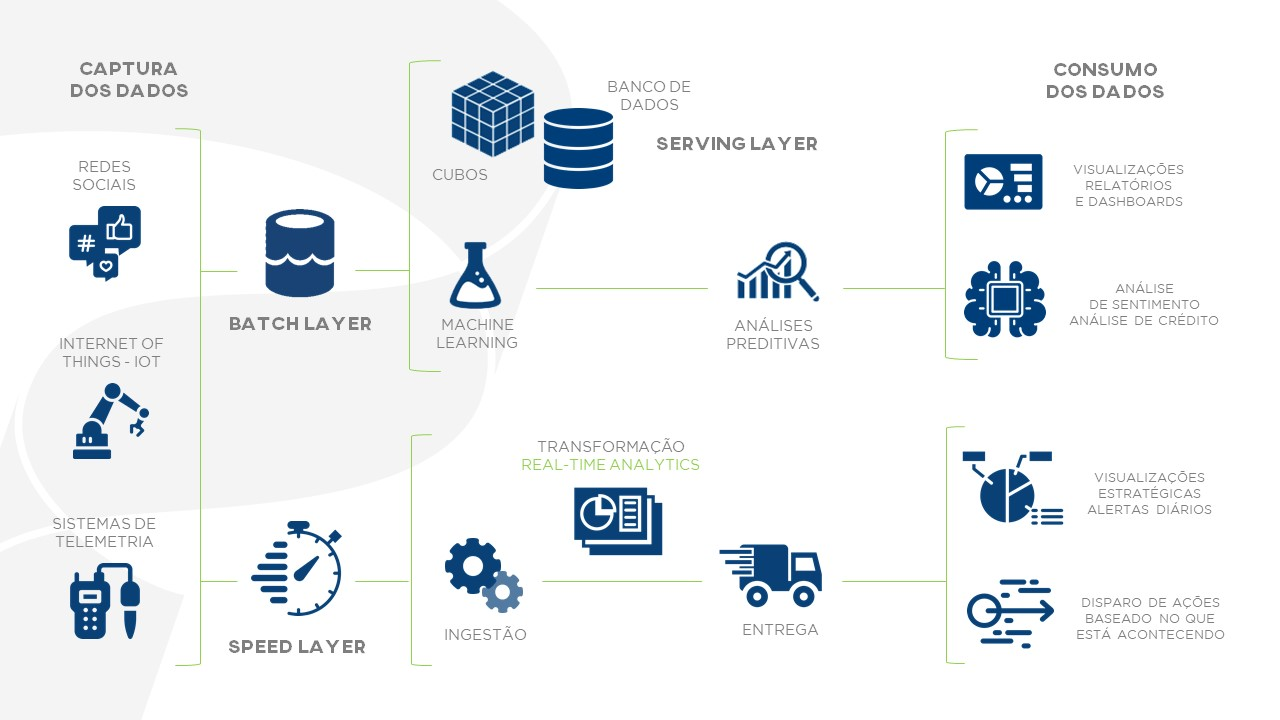
\includegraphics[width=0.7\textwidth]{imgs/img_001.jpg}
\caption{Exemplo de visualização dos resultados obtidos através da metodologia proposta. A figura ilustra o comportamento do sistema ao longo do tempo.}
\label{fig:exemplo}
\end{figure}

\subsection{Validação do Modelo}

\lipsum[11] A validação foi realizada comparando os resultados simulados com dados experimentais. O erro médio quadrático (RMSE) foi calculado através de:

\begin{equation}
RMSE = \sqrt{\frac{1}{n}\sum_{i=1}^{n}(y_i - \hat{y}_i)^2}
\label{eq:rmse}
\end{equation}

onde $y_i$ são os valores observados e $\hat{y}_i$ são os valores preditos pelo modelo.

% Resultados e Discussões
\section{Resultados e Discussões}

\lipsum[12-13] Os resultados obtidos demonstram a eficácia da metodologia proposta. A Tabela \ref{tab:resultados} apresenta uma comparação quantitativa entre diferentes abordagens.

\begin{table}[H]
\centering
\caption{Comparação de desempenho entre diferentes métodos}
\label{tab:resultados}
\begin{tabular}{@{}lccc@{}}
\toprule
\textbf{Método} & \textbf{RMSE} & \textbf{Tempo (s)} & \textbf{Precisão (\%)} \\ \midrule
Método Proposto & 0.0023 & 15.2 & 98.5 \\
Euler Clássico & 0.0145 & 8.7 & 92.3 \\
Runge-Kutta 4ª ordem & 0.0038 & 21.5 & 97.1 \\
Método Adaptativo & 0.0031 & 18.9 & 97.8 \\ \bottomrule
\end{tabular}
\end{table}

\subsection{Análise Quantitativa}

\lipsum[14] Os dados quantitativos revelam que o método proposto apresenta melhor desempenho em termos de precisão. A relação entre os parâmetros pode ser expressa por:

\begin{equation}
\eta = \frac{P_{out}}{P_{in}} \times 100\% = \frac{V_{out} \cdot I_{out}}{V_{in} \cdot I_{in}} \times 100\%
\label{eq:efficiency}
\end{equation}

onde $\eta$ representa a eficiência do sistema, $P_{out}$ é a potência de saída e $P_{in}$ é a potência de entrada.

\subsection{Análise Qualitativa}

\lipsum[15] Do ponto de vista qualitativo, observou-se que o comportamento do sistema é fortemente influenciado pelas condições iniciais e pelos parâmetros de controle. A matriz de transformação pode ser representada como:

\begin{equation}
\mathbf{A} = \begin{bmatrix}
a_{11} & a_{12} & a_{13} \\
a_{21} & a_{22} & a_{23} \\
a_{31} & a_{32} & a_{33}
\end{bmatrix}
\label{eq:matrix}
\end{equation}

\subsection{Discussão}

\lipsum[16-17] A análise dos resultados indica que a abordagem proposta oferece vantagens significativas em relação aos métodos tradicionais. Lorem ipsum dolor sit amet, consectetur adipiscing elit. Nullam in dui mauris. Vivamus hendrerit arcu sed erat molestie vehicula.

Proin adipiscing porta tellus, ut feugiat nibh adipiscing sit amet. In eu justo a felis faucibus ornare vel id metus. Vestibulum ante ipsum primis in faucibus orci luctus et ultrices posuere cubilia curae.

% Conclusão
\section{Conclusão}

\lipsum[18] Com base nos resultados obtidos, conclui-se que a metodologia desenvolvida apresenta excelente desempenho para análise de sistemas complexos. As principais contribuições deste trabalho incluem:

\begin{itemize}
    \item Desenvolvimento de um framework computacional robusto;
    \item Validação experimental dos modelos propostos;
    \item Comparação sistemática com métodos existentes;
    \item Identificação de limitações e oportunidades de melhoria.
\end{itemize}

Trabalhos futuros incluem a extensão da metodologia para sistemas multidimensionais e a incorporação de técnicas de otimização avançadas.

% Agradecimentos
\section*{Agradecimentos}

Os autores agradecem à Faculdade de Tecnologia do Estado de São Paulo (FATEC) e ao Centro Paula Souza (CPS) pelo apoio institucional. Este trabalho foi parcialmente financiado pela FAPESP (proc. 2024/12345-6) e CNPq (proc. 301234/2024-0).

% Referências
\bibliographystyle{IEEEtran}
\bibliography{referencias}

\end{document}
